\subsection{Spettro delle sorgenti a disposizione}

La nostra sorgente di \na{} ha 3 modi di decadimento:
\begin{itemize}
\item decadimento $\beta^+$ con $E_e=\SI{545}{keV}$, BR=90.4\% ed emissione di un fotone di energia \SI{1274}{keV} da parte del $^{22}$Ne formatosi;
\item cattura elettronica (BR=9.5\% ) con la conseguente emissione del fotone descritto sopra;
\item decadimento $\beta^-$ con BR=0.1\%.
\end{itemize}

Abbiamo a disposizione due sorgenti di \na{}: una con la stessa attività delle sorgenti di calibrazione, l'altra con un'attività molto maggiore.
Useremo i decadimenti $\gamma$ del \cs{} (\SI{662}{keV}) e del \co{} (\SI{1173}{keV}, \SI{1332}{keV}) per calibrare il nostro apparato.

\subsection{Processi di interesse}

Per misurare la massa dell'elettrone sfrutteremo il fatto che il positrone emesso dal decadimento $\beta^+$ del \na{}, avendo un'energia cinetica di circa \SI{30}{keV}, è quasi fermo. 
Una volta emesso interagisce con gli elettroni del sodio stesso producendo in modo isotropo una coppia di fotoni con impulsi uguali e opposti. L'energia di ogni fotone è uguale alla massa dell'elettrone. Questo processo può in realtà produrre un numero qualsiasi di fotoni. La probabilità decresce con l'aumentare di essi.

\marginpar{Approfondire la questione dei 3 fotoni\\
Non è inversamente proporzionale!}

\subsection{Fenomenologia dei rivelatori}

Nel range di energie dei fotoni in cui lavoriamo, i processi di diffusione possibili sono gli scattering Rayleigh e Compton e l'effetto fotoelettrico.
\marginpar{Diffusione???}
Lo scattering Rayleigh, in quanto completamente elastico, non rilascia energia nel calorimetro.
Nella diffusione Compton il fotone cede una parte dell'energia ad un elettrone del nostro calorimetro e possiamo misurare l'energia persa da quest'ultimo. La perdita di energia da parte del fotone non è monocromatica e segue una distribuzione denominata \emph{spalla Compton}.
Se il fotone esegue un effetto fotoelettrico, perde tutta la sua energia cedendola ad un elettrone ed è l'unico modo che abbiamo per conoscere l'energia del fotone incidente.

A questo quadro si possono aggiungere processi di ordine superiore, come un numero maggiore di rimbalzi Compton all'interno del cristallo oppure un effetto fotoelettrico eseguito dopo uno scattering Compton.
Vedremo in seguito che un fotone, dopo aver eseguito un Compton all'interno di un rivelatore, può uscirne ed essere rivelato anche da un altro.

Riportiamo in \autoref{sezioni} un grafico che rappresenta la sezione d'urto dell'effetto Compton confrontata con quella del fotoelettrico all'interno del NaI. Per energie minori di \SI{300}{keV} l'effetto fotoelettrico domina sul Compton e viceversa per energie maggiori.
Trascuriamo la produzione di coppie perché, quando è sopra soglia ($E_{\gamma}>\SI{1}{MeV}$), è 5 volte più piccola della sezione d'urto del fotoelettrico che, in questo range, è molto soppressa rispetto al Compton.

\begin{figure}[h]
\centering
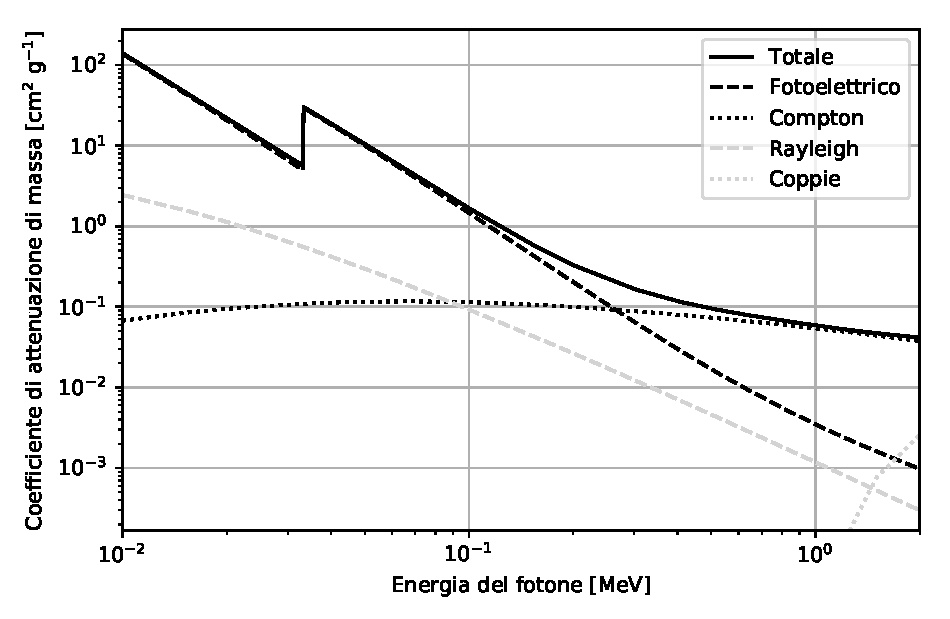
\includegraphics[width=25 em]{immagini/cross}
\caption{\label{fig:cross}
Coefficiente di attenuazione di massa in funzione dell'energia del fotone incidente all'interno del nostro cristallo di NaI ($\rho=\SI{3.67}{g\,cm^{-3}})$. Questa grandezza è definita come l'inverso di $\rho\lambda$, dove $\lambda$ è il cammino libero medio all'interno del materiale, quindi è proporzionale alla sezione d'urto. Queste informazioni sono tratte da \cite{cross}.}
\label{sezioni}
\end{figure}
